\section{Estructura}

\begin{tabular}{| c | c |}
    \hline
    Parte & Responsable \\ \hline
    Codigo Go & Frank Duarte \\ 
    Codigo c++ & Guillermo Caceres \\ 
    Codigo Python & Roger Infa \\ 
    Codigo Grafico & Roger Infa \\
    Informe & Roger Infa \\ \hline
\end{tabular}

\section{Introduccion}

En esta práctica se buscará  implementar satisfactoriamente dos algoritmos de ordenamiento, uno con tiempo computacional cuadrático y el otro con tiempo computacional logarítmico, esto con el fin de comprobar que  en algunos casos el uso de uno u otro método puede beneficiarnos hablando de costos computacionales ya sea para una cantidad  pequeña de datos o también para cantidades grandes.Además de ello, se compararán los tiempos de ejecucion entre tres lenguajes de programacion, estos son python,c++ y go.

Para la implementación de esta práctica se definirá el hardware  que usé para hacer todas las pruebas empezando por el Sistema Operativo, en este caso es  Windows 11. De procesador tengo un Intel 11th Gen Intel(R) Core(TM) i5-11400H @ 2.70GHz   2.69 GHz acompañado de 16.0 GB (15.8 GB usable) de RAM que trabajan con una frecuencia de  3.0GHz, con un disco sólido SSD de 512GB .

Estas prácticas fueron realizadas en los lenguajes de programación Python, c++ y go. Además de ello, se escogió Python para la generacion de graficos porque es fácil de entender e implementar graficos y es de tipado dinámico que en lo personal es fabuloso trabajar con un lenguaje así.

Para implementar los gráficos se tuvo que  instalar las librerías numpy y matplotlib con el comando \textbf{pip install  NOMBRE LIBRERIA }


\section{Algoritmos (los 02 algoritmos que va a implementar)}

Para hacer las comparaciones, hemos implementado un algoritmo de costo cuadratico y otro de costo logaritmico, estos son el bubble sort y merge sort respecticamente.

El bubble sort o tambien llamado ordenamiento de burbuja funciona marcando cada elemento de la lista que se odenará con el siguiente elemento y en cada "burbuja" intercambiara los elementos si es mayor que. Este algoritmo obtiene su nombre de la forma con la que suben por la lista los elementos durante los intercambios, como si fueran pequeñas "burbujas".

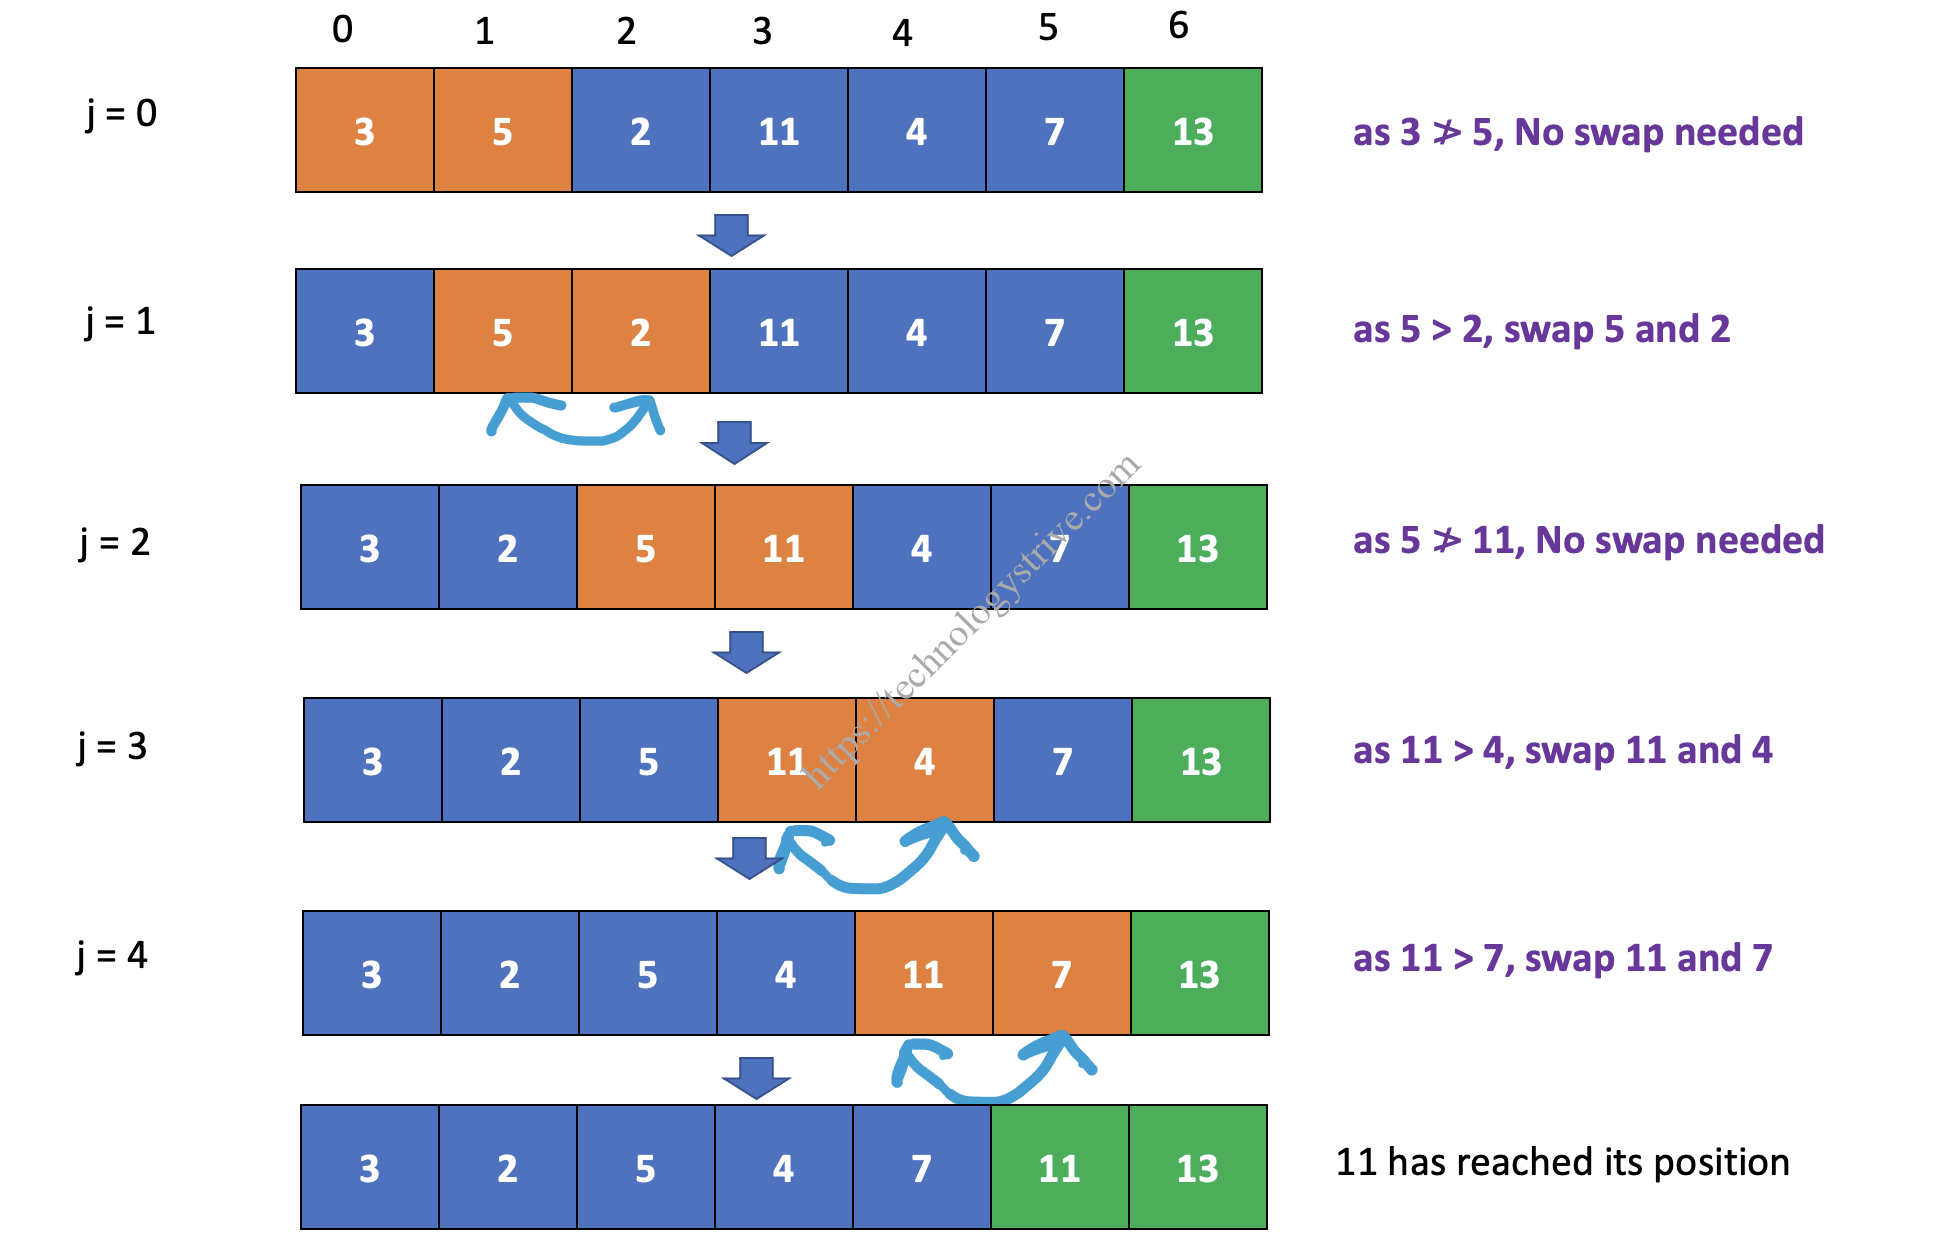
\includegraphics[width=12cm, center]{images/bubble.png}

El algoritmo Merge Sort es un algoritmo de clasificación que se basa en el paradigma divide y conquistaras. En este algoritmo, la matriz se divide inicialmente en dos mitades iguales y luego se combinan de manera ordenada utilizando comparaciones y recursividad.

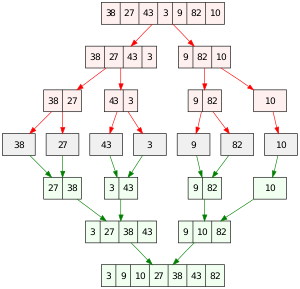
\includegraphics[width=10cm, center]{images/merge.png}
\section{Implementacion(codigo fuente)}
\section{Resultados}
\subsection{Tabla comparativa con el promedio de tiempo de procesamiento y desviacion estandar}
\subsection{Graficos}
\section{Conclusiones}

\textbf{SOLUCION:}
\begin{verbatim}
    // codigo
\end{verbatim}